\chapter{Stato dell'arte}\label{ch:chapter1}
Negli ultimi decenni, i progressi tecnologici nella miniaturizzazione dei dispositivi elettronici per l'elaborazione delle informazioni e i graduali processi di diffusione e di implementazione dei dispositivi di comunicazione wireless hanno contribuito notevolmente all'affermazione di una nuova realt� che facilmente si presta a numerosi impieghi: le reti di sensori wireless o WSN.
\newline
In questo capitolo vedremo come � caratterizzata una WSN e i suoi pregi e difetti. Vedremo il perch� Software Defined Networking, il quale verr� approfondito maggiormente nei capitoli successivi in merito alla sua architettura e le sue funzionalit�, � cos� importante per WSN e vedremo l'architettura che nasce dalla fusione di WSN con il protocollo. Infine verr� trattato un software simile al precedente: SDN-WISE, sul quale si basa il sistema realizzato.
\section{Wireless Sensor Network}
Con Wireless Sensor Network(WSN) si indica una topologia di rete informatica che, caratterizzata da una architettura distribuita, � costituita da un insieme di dispositivi elettronici autonomi in grado di prelevare dati dall'ambiente circostante e di comunicare tra loro.
In una rete WSN, ciascun sensore ha una regione di monitoraggio nel quale pu� monitorare eventi o oggetti nella regione. In aggiunta i sensori possono comunicare tra loro tramite interfacce che rientrano nella loro regione.
\newline
\begin{figure}[htbp]
\centering
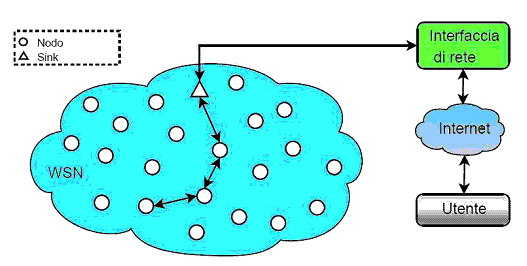
\includegraphics[width=0.95\textwidth,height=\textheight,keepaspectratio]{images/fig_1_1}
\caption{Rete WSN}
\label{fig:3_1}
\end{figure}
\newline
La comunicazione avviene in maniera asimmetrica, in quanto i nodi inviano i dati monitorati verso dei nodi speciali chiamati Sink, i quali sono gli unici nodi detta rete che si interfacciano con un calcolatore o un cloud. Le reti WSN devono avere diversi requisiti, fra i quali bassi consumi, scalabilit�, flessibilit� ed i nodi devono essere di piccole dimensioni ed a basso costo.
\subsection{Topologia di una WSN}
Le topologie di reti utilizzate in una WSN sono sostanzialmente tre:
\newline
- \textbf{Stella}: prevede un nodo centrale che funge da coordinatore della rete. Un qualsiasi altro nodo per comunicare con gli altri invia il messaggio al coordinatore che lo inoltra al destinatario; tutti i messaggi eseguono al massimo due hop. � la topologia pi� semplice che permette l'uso di protocolli e algoritmi altrettanto semplici.
\newline
- \textbf{Mesh}: nelle reti mesh o peer-to-peer ogni nodo della rete pu� comunicare con gli altri nodi della rete che rientrano nella sua copertura radio. I nodi sono considerati tutti uguali, perci� hanno tutti le stesse prestazioni. Viene definita \textit{multihop}, ovvero un messaggio pu� attraversare pi� nodi intermedi. I vantaggi sono che si possono creare reti pi� grandi e si possono avere percorsi ridondanti che aumentano affidabilit� e robustezza, introducendo per� algoritmi complessi.
\newline
- \textbf{Albero}: i nodi formano un albero. I messaggi partono da un nodo della rete e risalgono verso la radice, che raccoglie e dati e funge da coordinatore, ovvero il Sink. Il rischio pi� grande di questa topologia � proprio il sovraccarico del Sink.
\newline
\begin{figure}[htbp]
\centering
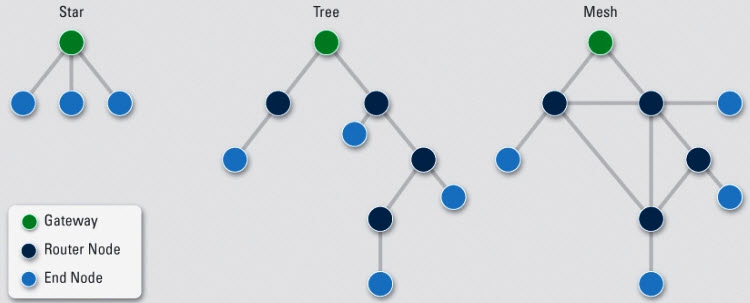
\includegraphics[width=0.95\textwidth,height=\textheight,keepaspectratio]{images/fig_1_2}
\caption{Topologie Rete WSN}
\label{fig:3_1}
\end{figure}
\newline

WSN ha un grandissimo potenziale ma ancora non ha raggiunto la sua efficacia ottimale. Ci� � dovuto alle sfide intrinseche presenti e la domanda crescente dalle applicazioni, il che ha portato ad aumentare l'interesse nella ricerca negli ultimi anni. Le maggiori sfide che dovr� affrontare WSN saranno sulla efficienza energetica, migliorare la comunicazione ed il routing.

\section{Software Defined Networking}
SDN � un paradigma il cui compito principale � quello di disaccoppiare le funzioni di controllo della rete da quelle di inoltro del traffico. Questo paradigma nasce proprio per risolvere i problemi delle reti tradizionali, ovvero la scarsa scalabilit� e complessit�, le quali non riuscivano a soddisfare le richieste di mercato dovute alla richiesta maggiore di applicazioni sempre pi� complesse ed un maggior numero di utilizzatori. 
\newline
Questo paradigma verr� abbondantemente trattato e definito in ogni sua sfaccettatura nei capitoli successivi. \cite{book}

\section{SDN-WISE}
SDN-WISE,� una soluzione Software Defined Network per Wireless Sensor Network. A differenza di SDN-WSN � stateful e propone due nuovi obbiettivi:
\newline
- riduzione di scambi di messaggi tra nodi e controller
\newline
- programmare i nodi come macchine a stati finiti cos� da poter abilitare operazioni che non potevano essere supportate da soluzioni stateless.
\subsection{Approccio SDN-WISE}
I Nodi di SDN-WISE sono racchiusi in tre strutture dati: WISE States Array, Accepted IDs Array e WISE Flow Table. Il Controller, come per l'approccio SDN, definisce le politiche di networking che verrano implementate dai vari sensori. In ogni momento i nodi SDN-WISE sono caratterizzati da uno stato corrente per ogni controller attivo. Il Wise States Array � una struttura dati che contiene il valore dello stato corrente.
\newline
In SDN-WISE, come nell'approccio SDN-WSN, � implementato il protocollo Sensor OverFlow (SOF) che permette ai nodi della rete di avere tabella di flusso (WISE Flow Table-WFT. Nel caso in cui un pacchetto venga processato, il sensore esplorer� le entries della WFT. Ciascuna entry of WFT contiene una sezione Matching Rules, nel quale vengono definite le condizioni per processare un pacchetto. In caso contrario il nodo richiede aiuto al controller. 
\newline
\newline
In SDN-WISE, la rete di sensori e i sink possono essere distinti. I Sink sono gateway tra il nodo sensore e il controller.
\newline
\begin{figure}[htbp]
\centering
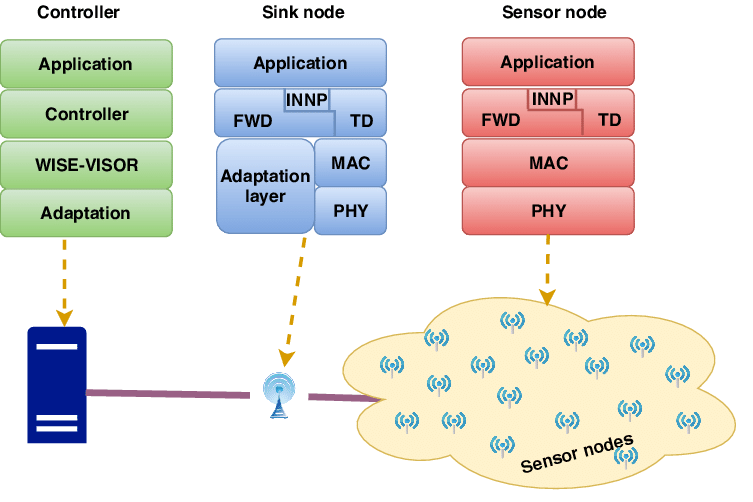
\includegraphics[width=0.95\textwidth,height=\textheight,keepaspectratio]{images/fig_1_3}
\caption{Architettura SDN-WISE}
\label{fig:3_1}
\end{figure}
\newline
I Pacchetti SDN-WISE hanno un header fissato, che consiste di 10 byte, divisi in vari campi come segue, figura:
\newline

\begin{figure}[htbp]
\centering
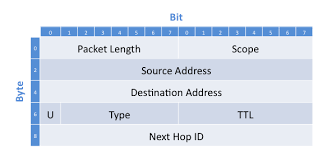
\includegraphics[width=0.95\textwidth,height=\textheight,keepaspectratio]{images/fig_1_4}
\caption{Header SDN-WISE}
\label{fig:3_1}
\end{figure}

- Il campo lunghezza del pacchetto contiene la lunghezza totale, incluso il payload, in bytes.
\newline
- Scope identifica un gruppo di Controller che hanno espresso interesse nel contenuto del pacchetto. Inizialmente � inizializzato a zero, ma pu� essere modificato attraverso appropriate entry della WFT.
\newline
- Indirizzo del Mittente e del Destinatario, come specificato nel nome, indicano gli indirizzi rispettivamente del nodo che ha generato il pacchetto e il nodo che lo riceve.











